% -*- latex -*-
%%%%%%%%%%%%%%%%%%%%%%%%%%%%%%%%%%%%%%%%%%%%%%%%%%%%%%%%%%%%%%%%
%%%%%%%%%%%%%%%%%%%%%%%%%%%%%%%%%%%%%%%%%%%%%%%%%%%%%%%%%%%%%%%%
%%%%
%%%% This text file is part of the lecture slides for
%%%% `Parallel Computing'
%%%% by Victor Eijkhout, copyright 2012-7
%%%%
%%%% MPIO-slides.tex : slides about MPI file I/O
%%%%
%%%%%%%%%%%%%%%%%%%%%%%%%%%%%%%%%%%%%%%%%%%%%%%%%%%%%%%%%%%%%%%%
%%%%%%%%%%%%%%%%%%%%%%%%%%%%%%%%%%%%%%%%%%%%%%%%%%%%%%%%%%%%%%%%

\begin{numberedframe}{Overview}
  This section discusses parallel I/O. What is the problem with
  regular I/O in parallel?

  Commands learned:
  \begin{itemize}
  \item \indexmpishow{MPI_File_open}\lstinline{/write/close} and variants
  \item parallel file pointer routines: \indexmpishow{MPI_File_set_view}\lstinline{/write_at}
  \end{itemize}
\end{numberedframe}

\begin{numberedframe}{The trouble with parallel I/O}
  \begin{itemize}
  \item Multiple process reads from one file: no problem.
  \item Multiple writes to one file: big problem.
  \item Everyone writes to separate file: stress on the file system,
    and requires post-processing.
  \end{itemize}
\end{numberedframe}

\begin{numberedframe}{MPI I/O}
  \begin{itemize}
  \item Part of MPI since MPI-2
  \item Joint creation of one file from bunch of processes.
  \item You could also use \n{hdf5}, \n{netcdf}, \n{silo}~\ldots
  \end{itemize}
\end{numberedframe}

\begin{numberedframe}{The usual bits}
\small
\lstset{language=C}
\begin{lstlisting}
MPI_File mpifile;
MPI_File_open(comm,"blockwrite.dat",
        MPI_MODE_CREATE | MPI_MODE_WRONLY,MPI_INFO_NULL,
        &mpifile);
if (procno==0) {
  MPI_File_write
    (mpifile,output_data,nwords,MPI_INT,MPI_STATUS_IGNORE);
}
MPI_File_close(&mpifile);
\end{lstlisting}
\lstset{language=Fortran}
\begin{lstlisting}
type(MPI_File) :: mpifile ! F08
integer        :: mpifile ! F90
\end{lstlisting}
\end{numberedframe}

\begin{numberedframe}{How do you make it unique for a process?}
\lstset{language=C}
\begin{lstlisting}
MPI_File_write_at
   (mpifile,offset,output_data,nwords,
    MPI_INT,MPI_STATUS_IGNORE);
\end{lstlisting}
or
\begin{lstlisting}
MPI_File_set_view
  (mpifile,
   offset,datatype,
   MPI_INT,"native",MPI_INFO_NULL);
MPI_File_write // no offset, we have a view
  (mpifile,output_data,nwords,MPI_INT,MPI_STATUS_IGNORE);
\end{lstlisting}
\end{numberedframe}

\begin{numberedframe}{Write at an offset}
  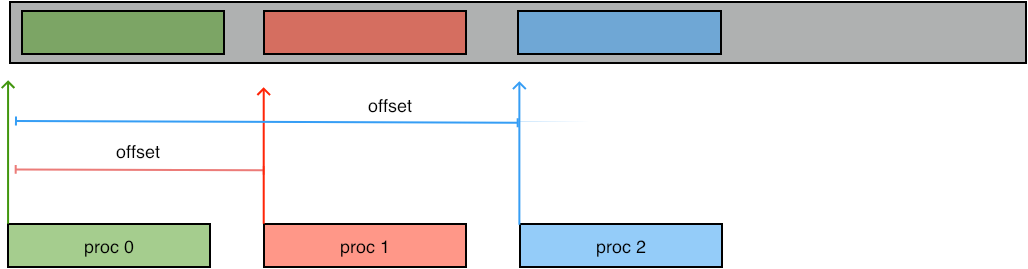
\includegraphics[scale=.35]{write-at-offset}
\end{numberedframe}

\begin{numberedframe}{Write to a view}
  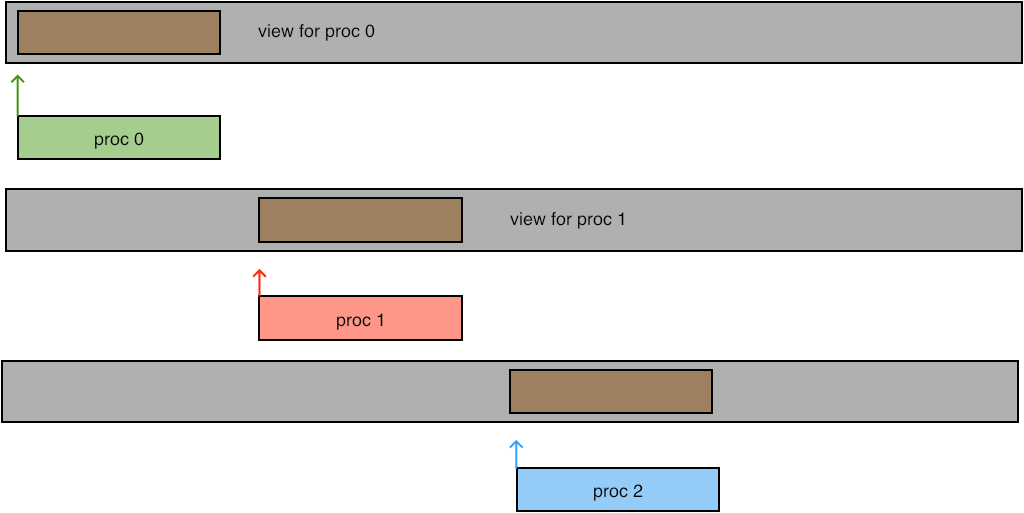
\includegraphics[scale=.35]{write-at-view}
\end{numberedframe}

\begin{numberedframe}{Write to a view}
  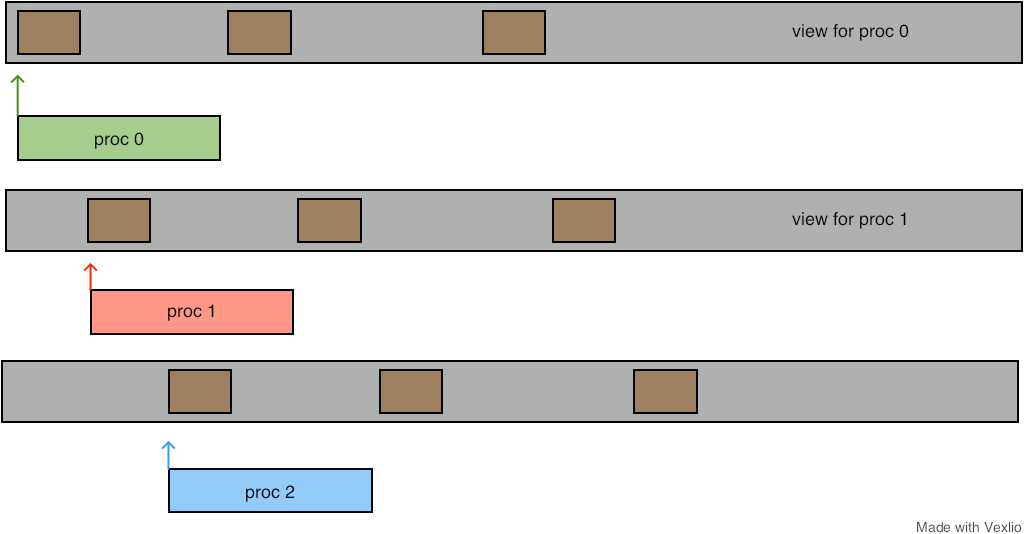
\includegraphics[scale=.35]{write-at-complicated}
\end{numberedframe}

\begin{exerciseframe}[blockwrite]
  The given code works for one writing process. Compute a unique
  offset for each process (in bytes!) so that all the local arrays are
  placed in the output file in sequence.
\end{exerciseframe}

\begin{exerciseframe}[viewwrite]
  Solve the previous exercise by using \indexmpishow{MPI_File_write} (that is,
  without offset), but by using \indexmpishow{MPI_File_set_view} to specify the location.
\end{exerciseframe}

\begin{exerciseframe}[scatterwrite]
  Now write the local arrays cyclically to the file: with 5~processes
  and 3~elements per process the file should contain
\begin{verbatim}
  1 4 7 10 13 | 2 5 8 11 14 | 3 6 9 12 15
\end{verbatim}
  Do this by defining a vector derived type and setting that as the
  file view.
\end{exerciseframe}

\endinput

\begin{numberedframe}{}
\begin{verbatim}

\end{verbatim}
\end{numberedframe}

